\begin{figure} \centering 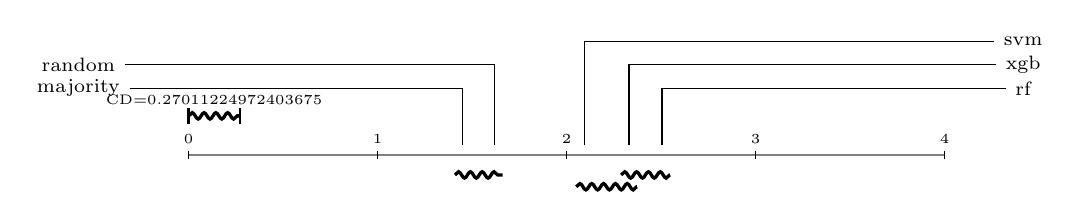
\begin{tikzpicture}[xscale=2]
\node (Label) at (1.362067349834422,0.7){\tiny{CD=0.27011224972403675}}; % the label
\draw[decorate,decoration={snake,amplitude=.4mm,segment length=1.5mm,post length=0mm}, very thick, color = black] (1.2,0.5) -- (1.524134699668844,0.5);
\foreach \x in {1.2,1.524134699668844} \draw[thick,color = black] (\x, 0.4) -- (\x, 0.6);
 
\draw[gray, thick](1.2,0) -- (6.0,0); 
\foreach \x in {1.2,2.4,3.6,4.8,6.0} \draw (\x cm,1.5pt) -- (\x cm, -1.5pt);
\node (Label) at (1.2,0.2){\tiny{0}};
\node (Label) at (2.4,0.2){\tiny{1}};
\node (Label) at (3.6,0.2){\tiny{2}};
\node (Label) at (4.8,0.2){\tiny{3}};
\node (Label) at (6.0,0.2){\tiny{4}};
\draw[decorate,decoration={snake,amplitude=.4mm,segment length=1.5mm,post length=0mm}, very thick, color = black](2.8911764705882357,-0.25) -- (3.194705882352941,-0.25);
\draw[decorate,decoration={snake,amplitude=.4mm,segment length=1.5mm,post length=0mm}, very thick, color = black](3.6617647058823533,-0.4) -- (4.0464705882352945,-0.4);
\draw[decorate,decoration={snake,amplitude=.4mm,segment length=1.5mm,post length=0mm}, very thick, color = black](3.946470588235295,-0.25) -- (4.2558823529411764,-0.25);
\node (Point) at (2.9411764705882355, 0){};  \node (Label) at (0.5,0.8500000000000001){\scriptsize{majority}}; \draw (Point) |- (Label);
\node (Point) at (3.144705882352941, 0){};  \node (Label) at (0.5,1.1500000000000001){\scriptsize{random}}; \draw (Point) |- (Label);
\node (Point) at (4.205882352941177, 0){};  \node (Label) at (6.5,0.8500000000000001){\scriptsize{rf}}; \draw (Point) |- (Label);
\node (Point) at (3.9964705882352947, 0){};  \node (Label) at (6.5,1.1500000000000001){\scriptsize{xgb}}; \draw (Point) |- (Label);
\node (Point) at (3.711764705882353, 0){};  \node (Label) at (6.5,1.4500000000000002){\scriptsize{svm}}; \draw (Point) |- (Label);
\end{tikzpicture}
\caption{Nemenyi post hoc test}
\label{fig:nemeny}
\end{figure}
